%%%%%%%%%%%%%%%%%%%%%%%%%%%%%%%%%%%%%%%%%
% Beamer Presentation
% LaTeX Template
% Version 2.0 (March 8, 2022)
%
% This template originates from:
% https://www.LaTeXTemplates.com
%
% Author:
% Vel (vel@latextemplates.com)
%
% License:
% CC BY-NC-SA 4.0 (https://creativecommons.org/licenses/by-nc-sa/4.0/)
%
%%%%%%%%%%%%%%%%%%%%%%%%%%%%%%%%%%%%%%%%%

%----------------------------------------------------------------------------------------
%	PACKAGES AND OTHER DOCUMENT CONFIGURATIONS
%----------------------------------------------------------------------------------------

\documentclass[
	11pt, % Set the default font size, options include: 8pt, 9pt, 10pt, 11pt, 12pt, 14pt, 17pt, 20pt
	%t, % Uncomment to vertically align all slide content to the top of the slide, rather than the default centered
	%aspectratio=169, % Uncomment to set the aspect ratio to a 16:9 ratio which matches the aspect ratio of 1080p and 4K screens and projectors
]{beamer}

\graphicspath{{Images/}{./}} % Specifies where to look for included images (trailing slash required)

\usepackage{booktabs} % Allows the use of \toprule, \midrule and \bottomrule for better rules in tables

%----------------------------------------------------------------------------------------
%	SELECT LAYOUT THEME
%----------------------------------------------------------------------------------------

% Beamer comes with a number of default layout themes which change the colors and layouts of slides. Below is a list of all themes available, uncomment each in turn to see what they look like.

%\usetheme{default}
%\usetheme{AnnArbor}
%\usetheme{Antibes}
%\usetheme{Bergen}
%\usetheme{Berkeley}
%\usetheme{Berlin}
%\usetheme{Boadilla}
%\usetheme{CambridgeUS}
%\usetheme{Copenhagen}
%\usetheme{Darmstadt}
%\usetheme{Dresden}
%\usetheme{Frankfurt}
%\usetheme{Goettingen}
%\usetheme{Hannover}
%\usetheme{Ilmenau}
%\usetheme{JuanLesPins}
%\usetheme{Luebeck}
\usetheme{Madrid}
%\usetheme{Malmoe}
%\usetheme{Marburg}
%\usetheme{Montpellier}
%\usetheme{PaloAlto}
%\usetheme{Pittsburgh}
%\usetheme{Rochester}
%\usetheme{Singapore}
%\usetheme{Szeged}
%\usetheme{Warsaw}

%----------------------------------------------------------------------------------------
%	SELECT COLOR THEME
%----------------------------------------------------------------------------------------

% Beamer comes with a number of color themes that can be applied to any layout theme to change its colors. Uncomment each of these in turn to see how they change the colors of your selected layout theme.

%\usecolortheme{albatross}
%\usecolortheme{beaver}
%\usecolortheme{beetle}
%\usecolortheme{crane}
%\usecolortheme{dolphin}
%\usecolortheme{dove}
%\usecolortheme{fly}
%\usecolortheme{lily}
%\usecolortheme{monarca}
%\usecolortheme{seagull}
%\usecolortheme{seahorse}
%\usecolortheme{spruce}
%\usecolortheme{whale}
%\usecolortheme{wolverine}
\usepackage{xcolor}

% Tsinghua purple
\definecolor{thupurple}{RGB}{102,8,116}

% Make it the structural color (titles, blocks, items, etc.)
\setbeamercolor{structure}{fg=thupurple}

% Optional: tidy up block colors to match
\setbeamercolor{block title}{bg=thupurple,fg=white}
\setbeamercolor{block body}{bg=thupurple!8,fg=black}
\setbeamercolor{frametitle}{bg=thupurple, fg=white}

%----------------------------------------------------------------------------------------
%	SELECT FONT THEME & FONTS
%----------------------------------------------------------------------------------------

% Beamer comes with several font themes to easily change the fonts used in various parts of the presentation. Review the comments beside each one to decide if you would like to use it. Note that additional options can be specified for several of these font themes, consult the beamer documentation for more information.

\usefonttheme{default} % Typeset using the default sans serif font
%\usefonttheme{serif} % Typeset using the default serif font (make sure a sans font isn't being set as the default font if you use this option!)
%\usefonttheme{structurebold} % Typeset important structure text (titles, headlines, footlines, sidebar, etc) in bold
%\usefonttheme{structureitalicserif} % Typeset important structure text (titles, headlines, footlines, sidebar, etc) in italic serif
%\usefonttheme{structuresmallcapsserif} % Typeset important structure text (titles, headlines, footlines, sidebar, etc) in small caps serif

%------------------------------------------------

%\usepackage{mathptmx} % Use the Times font for serif text
\usepackage{palatino} % Use the Palatino font for serif text

%\usepackage{helvet} % Use the Helvetica font for sans serif text
\usepackage[default]{opensans} % Use the Open Sans font for sans serif text
%\usepackage[default]{FiraSans} % Use the Fira Sans font for sans serif text
%\usepackage[default]{lato} % Use the Lato font for sans serif text

%----------------------------------------------------------------------------------------
%	SELECT INNER THEME
%----------------------------------------------------------------------------------------

% Inner themes change the styling of internal slide elements, for example: bullet points, blocks, bibliography entries, title pages, theorems, etc. Uncomment each theme in turn to see what changes it makes to your presentation.

%\useinnertheme{default}
\useinnertheme{circles}
%\useinnertheme{rectangles}
%\useinnertheme{rounded}
%\useinnertheme{inmargin}

%----------------------------------------------------------------------------------------
%	SELECT OUTER THEME
%----------------------------------------------------------------------------------------

% Outer themes change the overall layout of slides, such as: header and footer lines, sidebars and slide titles. Uncomment each theme in turn to see what changes it makes to your presentation.

%\useoutertheme{default}
%\useoutertheme{infolines}
%\useoutertheme{miniframes}
%\useoutertheme{smoothbars}
%\useoutertheme{sidebar}
%\useoutertheme{split}
%\useoutertheme{shadow}
%\useoutertheme{tree}
%\useoutertheme{smoothtree}

%\setbeamertemplate{footline} % Uncomment this line to remove the footer line in all slides
%\setbeamertemplate{footline}[page number] % Uncomment this line to replace the footer line in all slides with a simple slide count

%\setbeamertemplate{navigation symbols}{} % Uncomment this line to remove the navigation symbols from the bottom of all slides

\usepackage{CJKutf8}
\newcommand{\cn}[1]{\begin{CJK}{UTF8}{gbsn}#1\end{CJK}}

%----------------------------------------------------------------------------------------
%	PRESENTATION INFORMATION
%----------------------------------------------------------------------------------------

\title[Self-Resolving Prediction markets]{Self-Resolving Prediction Markets for
Unverifiable Outcomes} % The short title in the optional parameter appears at the bottom of every slide, the full title in the main parameter is only on the title page

\subtitle{} % Presentation subtitle, remove this command if a subtitle isn't required

\author[\cn{威廉}]{Vilhjalmur A. Vilhjalmsson (\cn{威廉})} % Presenter name(s), the optional parameter can contain a shortened version to appear on the bottom of every slide, while the main parameter will appear on the title slide

\institute[UC]{Tsinghua University \\ \smallskip \textit{weil25@mails.tsinghua.edu.cn}} % Your institution, the optional parameter can be used for the institution shorthand and will appear on the bottom of every slide after author names, while the required parameter is used on the title slide and can include your email address or additional information on separate lines

\date[\today]{Algorithm Economics (80470223-0) - Course Project \\ \today} % Presentation date or conference/meeting name, the optional parameter can contain a shortened version to appear on the bottom of every slide, while the required parameter value is output to the title slide

%----------------------------------------------------------------------------------------

\begin{document}

%----------------------------------------------------------------------------------------
%	TITLE SLIDE
%----------------------------------------------------------------------------------------

\begin{frame}
	\titlepage % Output the title slide, automatically created using the text entered in the PRESENTATION INFORMATION block above
\end{frame}

%----------------------------------------------------------------------------------------
%	TABLE OF CONTENTS SLIDE
%----------------------------------------------------------------------------------------

% The table of contents outputs the sections and subsections that appear in your presentation, specified with the standard \section and \subsection commands. You may either display all sections and subsections on one slide with \tableofcontents, or display each section at a time on subsequent slides with \tableofcontents[pausesections]. The latter is useful if you want to step through each section and mention what you will discuss.

\begin{frame}
	\frametitle{Presentation Overview} % Slide title, remove this command for no title
	
	\tableofcontents % Output the table of contents (all sections on one slide)
	%\tableofcontents[pausesections] % Output the table of contents (break sections up across separate slides)
\end{frame}

%----------------------------------------------------------------------------------------
%	PRESENTATION BODY SLIDES
%----------------------------------------------------------------------------------------
\section{Introduction}
\begin{frame}
	\frametitle{Introduction}
	\begin{columns}[c] % "c" = vertically centered; use "t" to top-align both columns
		\begin{column}{0.55\textwidth} % Left column: bullet points
			\begin{itemize}
				\item Name: Self-Resolving Prediction Markets for
				Unverifiable Outcomes
				\item Main Topics:
				\begin{itemize}
					\item Prediction Markets
					\item Mechanism Design
					\item Information Aggregation
					\item Peer Prediction
					\item Information Elicitation
				\end{itemize}
			\end{itemize}
		\end{column}
		\begin{column}{0.4\textwidth} % Right column: image
			\begin{figure}
				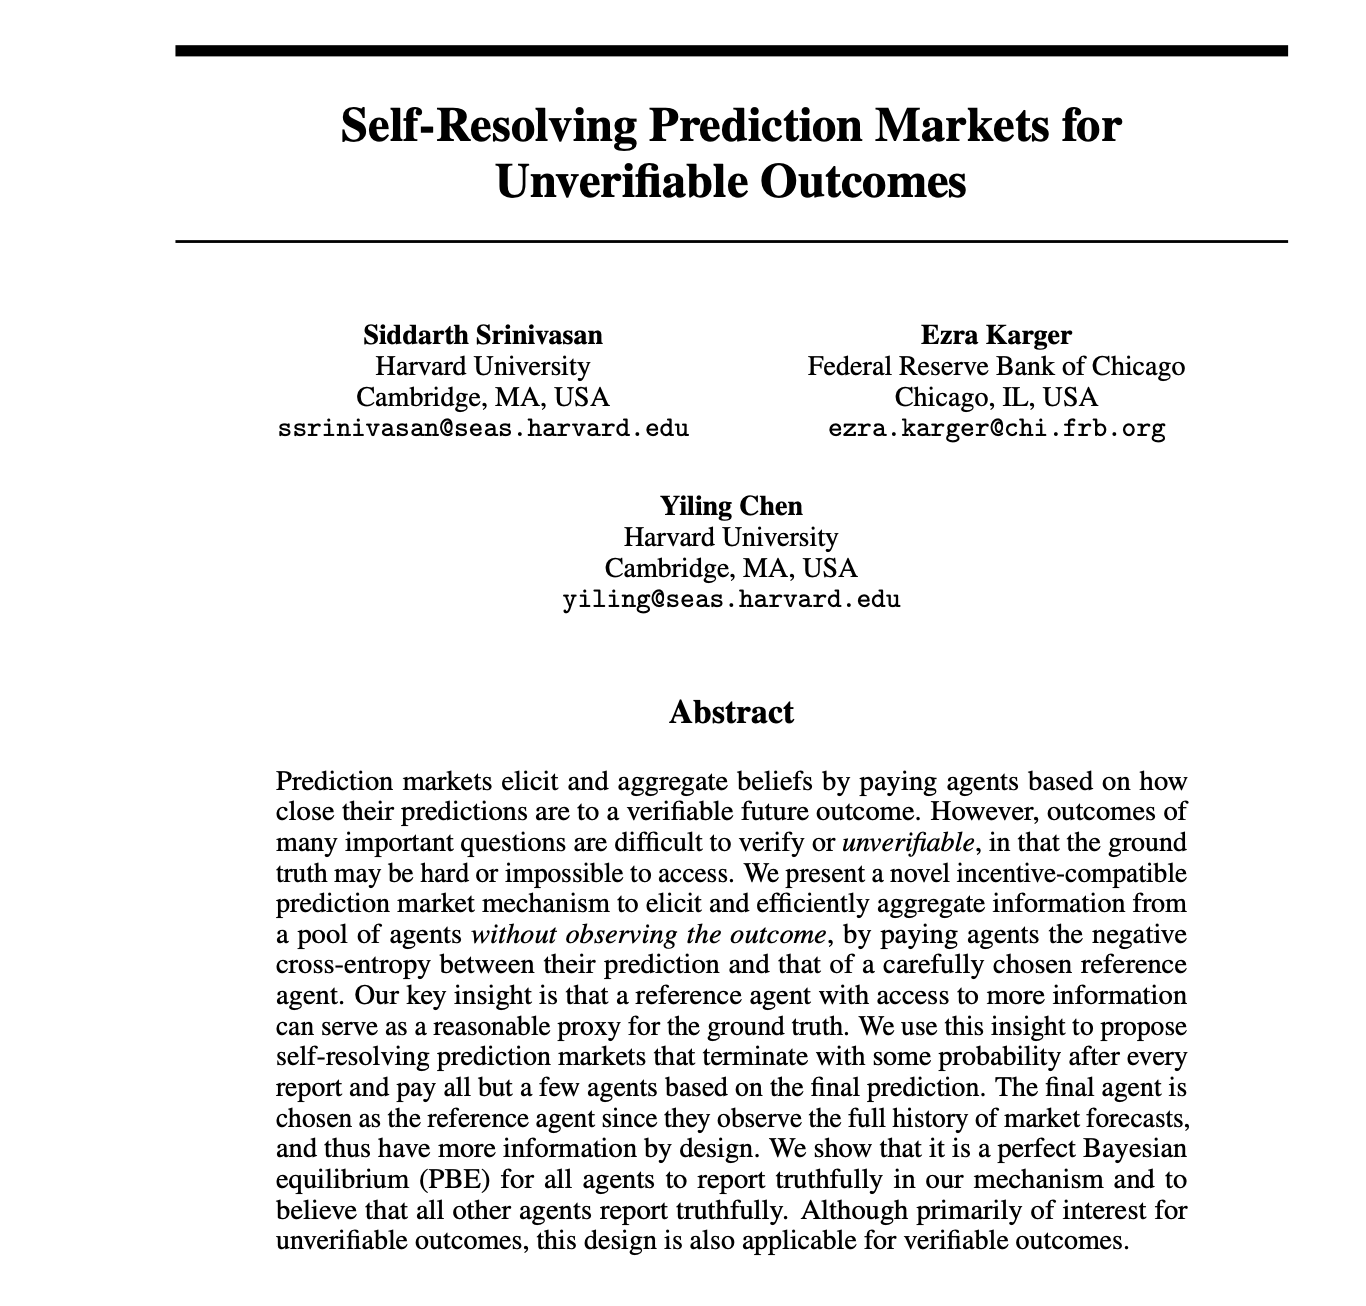
\includegraphics[width=\linewidth]{Images/paper_cover.png}
				\caption{Paper cover.} % Remove this line if no caption wanted
			\end{figure}
		\end{column}
	\end{columns}
	
\end{frame}

\section{Motivation and Problem Setup}
\begin{frame}
	\frametitle{Motivation and Problem Setup}

	\begin{itemize}
		\setlength{\itemsep}{1.5em} % space between the main bullets
		\item Prediction Markets are excellent at forecasting things that eventually resolve.
		\begin{itemize}
			\item Pay people once the truth is revealed.
			\item E.g., elections, sports, disease spread
		\end{itemize}
		\item What about questions that don't resolve cleanly?
		\begin{itemize}
			\item E.g., Content moderation decisions, Causal effects of policies
		\end{itemize}
	\end{itemize}
	
\end{frame}

\begin{frame}
	\frametitle{Motivation and Problem Setup}
	
	\begin{block}{Key Idea}
		Can we replace the verifiable outcome with a reference agent that has more information about the outcome?
	\end{block}
\end{frame}

\section{Background}

\begin{frame}
	\frametitle{What is a Prediction Market?}
	
	\begin{definition}[What is a Prediction Market]
		A prediction market is a mechanism that allows people to bet on the outcome of an event.
	\end{definition}

	\begin{example}
		\begin{itemize}
			\item Polymarket
			\item The stock market
			\item Sport betting
		\end{itemize}
	\end{example}

\end{frame}

\begin{frame}
	\frametitle{Background: Scoring Rules}

	\begin{block}{Idea}
		A \alert{(proper) scoring rule} pays an agent for a probabilistic
		prediction so that reporting their \emph{true belief} maximizes their
		expected payoff.
	\end{block}

	\vspace{0.5em}
	\begin{itemize}
		\item \alert{Problem:} this requires observing the outcome $i$.
	\end{itemize}

	\begin{definition}[Cross-Entropy Scoring Rule]
		Score a report $q$ against a \alert{reference prediction}
		$r \in \Delta\Omega_Y$ instead of an outcome:
		$$
		S_{CE}(r, q) = -H(r, q) = \sum_{i=1}^{Y} r_i \log q_i .
		$$
	\end{definition}

\end{frame}

\begin{frame}
	\frametitle{Background: The Key Swap}

	\begin{columns}[t]
		\begin{column}{0.48\textwidth}
			\begin{block}{Standard scoring rule}
				\centering
				prediction \quad vs. \quad \alert{outcome}
				\vspace{0.5em}
				$$ S(i, q) = \log q_i $$
				\vspace{0.3em}
				\emph{Needs the truth to be revealed.}
			\end{block}
		\end{column}
		\begin{column}{0.48\textwidth}
			\begin{block}{Cross-entropy scoring rule}
				\centering
				prediction \quad vs. \quad \alert{reference}
				\vspace{0.5em}
				$$ S_{CE}(r, q) = \sum_i r_i \log q_i $$
				\vspace{0.3em}
				\emph{Needs a reference prediction $r$.}
			\end{block}
		\end{column}
	\end{columns}

	\vspace{1em}
	\centering
	\small This swap is what lets the market resolve \emph{without an outcome}.
\end{frame}


\begin{frame}
	\frametitle{The Self-Resolving Prediction Market Mechanism}
	
	\begin{itemize}
		\item Consider a prediction market for a binary outcome $Y \in \{0,1\}$ with a common prior $\pi$.
		\item $M$ agents arrive in sequence.
		\item Each agent has a private signal $s_i \in [0,1]$ that is conditionally independent of the others given $Y$.
		\item Each agent sees the previous market report plus its own signal, forms a belief, and reports it.
		\item The market terminates with probability $\alpha$ after each report; the terminal agent is the reference.
		\item Agents $1..T-k$ are paid the cross-entropy market scoring rule against the reference, and the last $k$ agents receive a flat fee $R$.
	\end{itemize}
\end{frame}

\begin{frame}
	\frametitle{The Self-Resolving Prediction Market Mechanism}
	\begin{figure}
		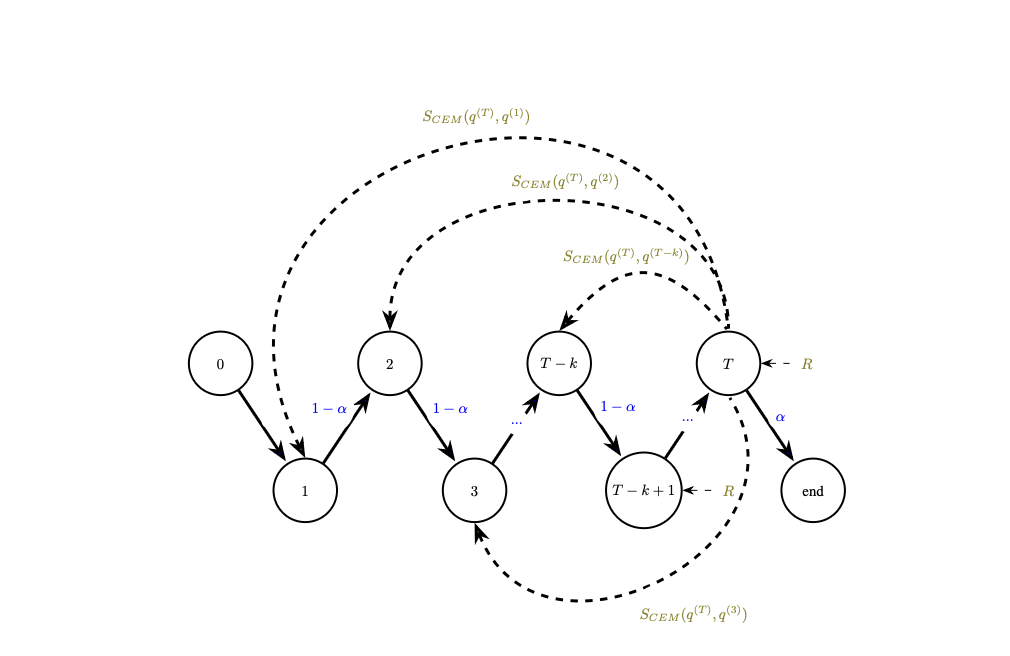
\includegraphics[width=0.8\linewidth]{Images/srpm_mechanism.png}
		\caption{The Self-Resolving Prediction Market Mechanism.}
	\end{figure}
\end{frame}

\begin{frame}
	\frametitle{Scoring rule in mechanism}
	\begin{itemize}
		\item The scoring rule in the mechanism is the CE-MSR.
		\item The scoring rule is defined as:
		$$
		S_{CEM}(q^t, q^{t-1}, r) = -H(r, q^t) + H(r, q^{t-1}) = \sum_{i=1}^Y r_i \log \frac{q^t_i}{q^{t-1}_i}
		$$
		\item Intuition: how much better is the new report than the previous one, compared to the reference?
	\end{itemize}

\end{frame}

\section{Limitations and Proposed Research Questions}
\begin{frame}
	\frametitle{Limitations and Proposed Research Questions}

	The paper's incentive guarantees are \emph{theoretical}: they rest on the reference being a good proxy for the truth, and the mechanism is never tested on real data.

	\medskip
	\begin{block}{RQ1 --- Simulation (incentives)}
		Under strategic deviation, \emph{when} is truthful reporting a best response, and how does this depend on how well-informed the reference is?
	\end{block}

	\begin{block}{RQ2 --- Empirical (real markets)}
		How closely do self-resolving payouts track the standard verifiable (outcome-based) payouts on resolved real-world markets?
	\end{block}
\end{frame}

%------------------------------------------------

\section{Experiments and Results}

\subsection{Simulation Study}

\begin{frame}
	\frametitle{RQ1 Preliminaries: The Three Knobs}
	\framesubtitle{What the simulation actually varies}
	\small

	\begin{block}{The paper's informativeness parameters (Assumption 5)}
		\begin{itemize}
			\item $\delta$ --- \alert{how informative} a signal is.
			Via the Bhattacharyya coefficient, $\delta = 1-\mathrm{BC}$:
			$\delta = 0$ means $P(X\mid Y{=}0)=P(X\mid Y{=}1)$ (useless);
			larger $\delta$ separates the two classes.
			\item $\eta$ --- a \alert{floor on signal probabilities},
			$\min_{x,\omega} P(X{=}x\mid Y{=}\omega)\ge\eta$.
			No signal is arbitrarily decisive ($\eta$ bounds how far one report can move a belief).
		\end{itemize}
	\end{block}

	\begin{block}{Our deviation parameter (simulation construct)}
		$\gamma$ scales the focal agent's signal: report
		$\mathrm{logit}(\pi) + \gamma\,\ell$.
		$\gamma=1$ truthful, $\gamma>1$ over-confident.
	\end{block}

	\centering
	\alert{Link:} the theory bounds the \emph{gain} from any deviation
	($D_\eta(\Delta,\mathbf{y})$, Thm.~3) and shows it $\to 0$ as $k$ grows.
	$\gamma$ is how we \emph{realize} a deviation; $\gamma^\star\!\to\!1$ is that bound biting.
\end{frame}

\begin{frame}
	\frametitle{RQ1 (Simulation): Is Truthful Reporting a Best Response?}

	\textbf{Setup --- an agent-based simulator of the mechanism}
	\begin{itemize}
		\item Binary $Y$, conditionally independent signals, payment via CE-MSR against the terminal \emph{reference} agent.
		\item A focal agent deviates by scaling its signal: it reports $\mathrm{logit}(\pi) + \gamma\,\ell$, where $\ell$ is its log-likelihood ratio. $\gamma=1$ is truthful, $\gamma>1$ over-confident.
		\item The reference observes the focal report \emph{plus} $k$ independent signals (its informational substitutes).
		\item Sweep $k \in \{0,2,8,32,64,128,256\}$ and estimate the profit-maximising $\gamma^\star$ by Monte Carlo ($4\times 10^5$ samples).
	\end{itemize}

	\begin{block}{Hypothesis}
		Few substitutes $\Rightarrow$ it pays to over-report ($\gamma^\star>1$); as $k$ grows the reference $\approx$ ground truth, so $\gamma^\star \to 1$ (truthful).
	\end{block}
\end{frame}

%------------------------------------------------

\begin{frame}
	\frametitle{RQ1 Results: Truthfulness Needs an Informed Reference}

	\begin{columns}[c]
		\begin{column}{0.62\textwidth}
			\begin{figure}
				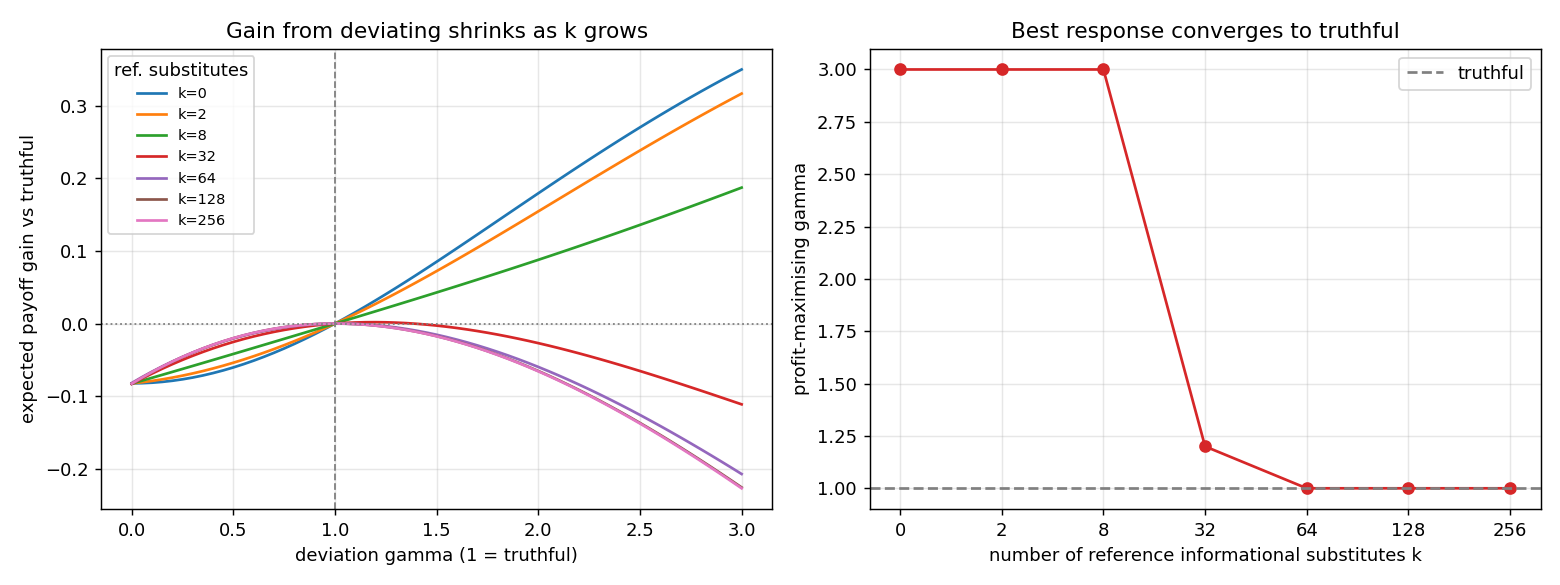
\includegraphics[width=\linewidth]{Images/sim_incentives.png}
			\end{figure}
		\end{column}
		\begin{column}{0.38\textwidth}
			\begin{itemize}
				\item $k \le 8$: best response is to grossly over-report ($\gamma^\star = 3$).
				\item $k = 32$: $\gamma^\star \approx 1.2$.
				\item $k \ge 64$: $\gamma^\star = 1.0$ --- \alert{exactly truthful}.
			\end{itemize}
			\medskip
			Matches Theorems 1--3: truthfulness emerges once the reference has enough informational substitutes.
		\end{column}
	\end{columns}

	\smallskip
	{\footnotesize Aside: under truthful play the market reproduces the full-information Bayesian posterior (gap $\sim 10^{-13}$).}
\end{frame}

%------------------------------------------------

\subsection{Empirical Study}

\begin{frame}
	\frametitle{RQ2 (Empirical): Counterfactual on Real Polymarket Data}

	\textbf{Data \& method} --- $\sim$90 resolved markets (volume $> \$100$k).
	\begin{itemize}
		\item Treat the Yes-price path as sequential reports $q^{(t)}=[1-p_t,\,p_t]$; each price move is a ``reporter''.
		\item Pay the \emph{same} transitions two ways:
		\begin{itemize}
			\item \textbf{Self-resolving}: CE-MSR against a late reference price $r$ (no outcome needed).
			\item \textbf{Verifiable}: log-MSR against the realised outcome $Y$.
		\end{itemize}
		\item Sweep how ``late'' $r$ is: \texttt{lead\_1h/24h/168h} (before close), \texttt{life\_50pct} (halfway through the market's life), \texttt{window\_1-24h} (averaged late window).
		\item Compare payout correlation, top-decile reporter overlap, and total payout ratio.
	\end{itemize}
\end{frame}

%------------------------------------------------

\begin{frame}
	\frametitle{RQ2 Results: Payouts Track; Leakage Drives the Gap}

	\begin{columns}[c]
		\begin{column}{0.55\textwidth}
			\begin{figure}
				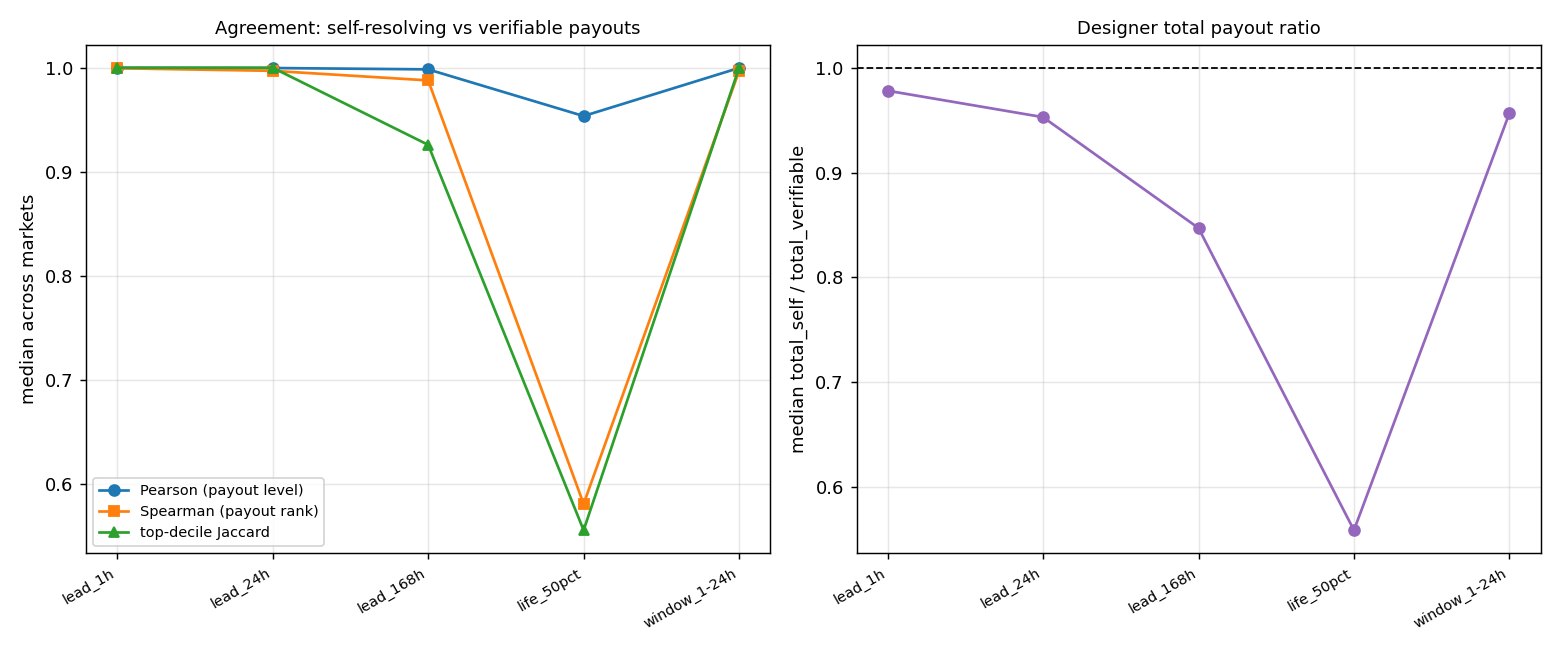
\includegraphics[width=\linewidth]{Images/emp_reference_sweep.png}
			\end{figure}
		\end{column}
		\begin{column}{0.45\textwidth}
			\scriptsize
			\setlength{\tabcolsep}{3.5pt}
			\begin{tabular}{lccc}
				\toprule
				ref. & Pears. & Spear. & ratio \\
				\midrule
				lead\_1h    & 1.00 & 1.00 & 0.98 \\
				lead\_24h   & 1.00 & 1.00 & 0.95 \\
				lead\_168h  & 1.00 & 0.99 & 0.85 \\
				life\_50pct & 0.95 & 0.58 & 0.56 \\
				window      & 1.00 & 1.00 & 0.96 \\
				\bottomrule
			\end{tabular}

			\smallskip
			\textbf{Pearson}: do payout \emph{amounts} agree?\\
			\textbf{Spearman}: does the \emph{ranking} (who earns most) agree?

			\smallskip
			Amounts track almost perfectly; ranking degrades as $r$ moves earlier --- that gap is outcome leakage.
		\end{column}
	\end{columns}

	\smallskip
	{\footnotesize Measures whether the \emph{outputs} match (not incentive compatibility) --- complementary to RQ1.}
\end{frame}

%------------------------------------------------

\begin{frame}
	\frametitle{RQ2: Worked Example --- Kamala Harris Popular-Vote Market}

	\begin{columns}[c]
		\begin{column}{0.64\textwidth}
			\begin{figure}
				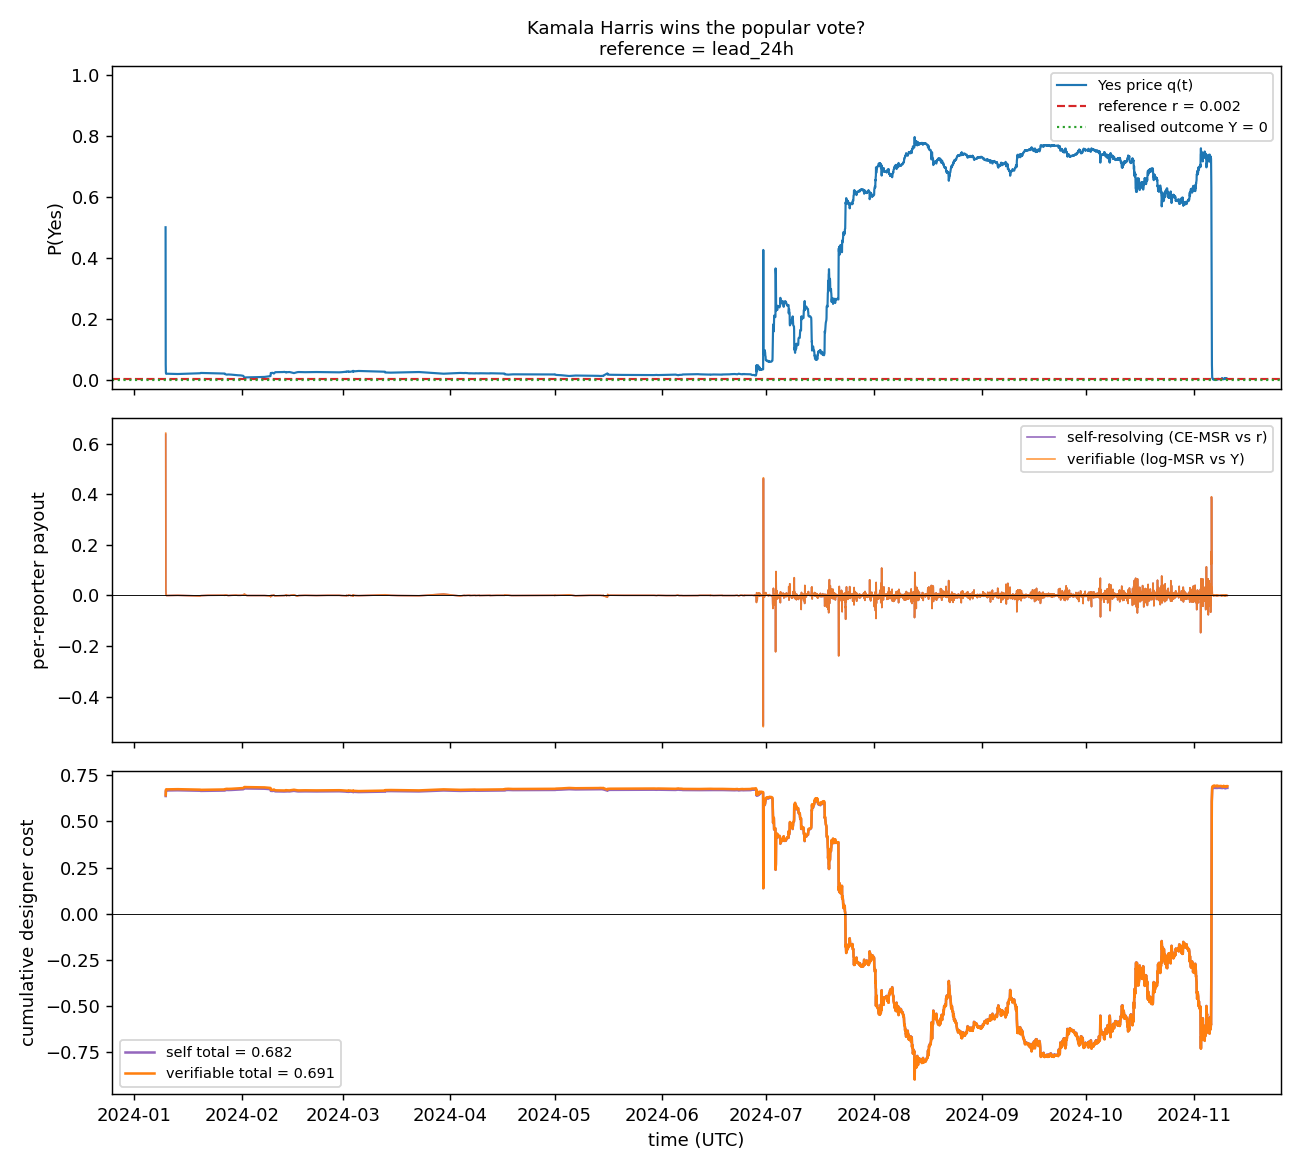
\includegraphics[width=\linewidth]{Images/emp_example_kamala.png}
			\end{figure}
		\end{column}
		\begin{column}{0.36\textwidth}
			\footnotesize
			A high-volume market ($\sim$2{,}700 price moves, outcome $Y=0$).
			\smallskip

			The self-resolving payouts (CE-MSR vs.\ the 24h reference) and the verifiable payouts (vs.\ the outcome) are \alert{visually indistinguishable}.
			\medskip

			\centering
			\begin{tabular}{lc}
				\toprule
				Pearson & $1.00$ \\
				Spearman & $1.00$ \\
				payout ratio & $0.99$ \\
				\midrule
				self total & $0.68$ \\
				verifiable total & $0.69$ \\
				\bottomrule
			\end{tabular}
		\end{column}
	\end{columns}
\end{frame}

%------------------------------------------------

\begin{frame}
	\frametitle{RQ2: Per-Market Agreement (High-Volume Markets)}

	Pearson / Spearman of per-reporter payouts at a \emph{late} reference (24h before close) vs.\ a \emph{mid-life} reference (halfway through the market):

	\medskip
	\begin{table}
		\centering
		\footnotesize
		\setlength{\tabcolsep}{6pt}
		\begin{tabular}{lccccc}
			\toprule
			& & \multicolumn{2}{c}{late (24h)} & \multicolumn{2}{c}{mid-life (50\%)} \\
			\cmidrule(lr){3-4}\cmidrule(lr){5-6}
			Market & \#rep & P & S & P & S \\
			\midrule
			Kamala popular vote        & 2681 & 1.00 & 1.00 & 1.00 & 0.45 \\
			Poilievre next Canadian PM & 1030 & 1.00 & 1.00 & 0.96 & 0.91 \\
			Russia--Ukraine ceasefire '25 & 2531 & 1.00 & 1.00 & 0.99 & 0.98 \\
			US government shutdown     &  778 & 1.00 & 1.00 & 0.41 & $-0.48$ \\
			TikTok ban (May '25)       & 1078 & 1.00 & 1.00 & $-0.37$ & $-0.54$ \\
			\bottomrule
		\end{tabular}
	\end{table}

	\medskip
	{\footnotesize At a genuinely \emph{late} reference every market tracks perfectly. At \emph{mid-life}, some still track (ceasefire, Poilievre) while others collapse (shutdown, TikTok) --- the more the late price already leaks the outcome, the larger the gap.}
\end{frame}

%------------------------------------------------


\section{Text Examples} % Sections are added in order to organize your presentation into discrete blocks, all sections and subsections are automatically output to the table of contents as an overview of the talk but NOT output in the presentation as separate slides

\subsection{Paragraphs and Lists}

\begin{frame}
	\frametitle{Paragraphs of Text}
	
	Sed iaculis \alert{dapibus gravida}. Morbi sed tortor erat, nec interdum arcu. Sed id lorem lectus. Quisque viverra augue id sem ornare non aliquam nibh tristique. Aenean in ligula nisl. Nulla sed tellus ipsum. Donec vestibulum ligula non lorem vulputate fermentum accumsan neque mollis.
	
	\bigskip % Vertical whitespace
	
	% Quote example
	\begin{quote}
		Sed diam enim, sagittis nec condimentum sit amet, ullamcorper sit amet libero. Aliquam vel dui orci, a porta odio.\\
		--- Someone, somewhere\ldots
	\end{quote}
	
	\bigskip % Vertical whitespace
	
	Nullam id suscipit ipsum. Aenean lobortis commodo sem, ut commodo leo gravida vitae. Pellentesque vehicula ante iaculis arcu pretium rutrum eget sit amet purus. Integer ornare nulla quis neque ultrices lobortis.
\end{frame}

%------------------------------------------------

\begin{frame}
	\frametitle{Lists}
	\framesubtitle{Bullet Points and Numbered Lists} % Optional subtitle
	
	\begin{itemize}
		\item Lorem ipsum dolor sit amet, consectetur adipiscing elit
		\item Aliquam blandit faucibus nisi, sit amet dapibus enim tempus
		\begin{itemize}
			\item Lorem ipsum dolor sit amet, consectetur adipiscing elit
			\item Nam cursus est eget velit posuere pellentesque
		\end{itemize}
		\item Nulla commodo, erat quis gravida posuere, elit lacus lobortis est, quis porttitor odio mauris at libero
	\end{itemize}
	
	\bigskip % Vertical whitespace
	
	\begin{enumerate}
		\item Nam cursus est eget velit posuere pellentesque
		\item Vestibulum faucibus velit a augue condimentum quis convallis nulla gravida 
	\end{enumerate}
\end{frame}

%------------------------------------------------

\subsection{Blocks}

\begin{frame}
	\frametitle{Blocks of Highlighted Text}
	
	\begin{block}{Block Title}
		Lorem ipsum dolor sit amet, consectetur adipiscing elit. Integer lectus nisl, ultricies in feugiat rutrum, porttitor sit amet augue.
	\end{block}
	
	\begin{exampleblock}{Example Block Title}
		Aliquam ut tortor mauris. Sed volutpat ante purus, quis accumsan.
	\end{exampleblock}
	
	\begin{alertblock}{Alert Block Title}
		Pellentesque sed tellus purus. Class aptent taciti sociosqu ad litora torquent per conubia nostra, per inceptos himenaeos.
	\end{alertblock}
	
	\begin{block}{} % Block without title
		Suspendisse tincidunt sagittis gravida. Curabitur condimentum, enim sed venenatis rutrum, ipsum neque consectetur orci.
	\end{block}
\end{frame}

%------------------------------------------------

\subsection{Columns}

\begin{frame}
	\frametitle{Multiple Columns}
	\framesubtitle{Subtitle} % Optional subtitle
	
	\begin{columns}[c] % The "c" option specifies centered vertical alignment while the "t" option is used for top vertical alignment
		\begin{column}{0.45\textwidth} % Left column width
			\textbf{Heading}
			\begin{enumerate}
				\item Statement
				\item Explanation
				\item Example
			\end{enumerate}
		\end{column}
		\begin{column}{0.5\textwidth} % Right column width
			Lorem ipsum dolor sit amet, consectetur adipiscing elit. Integer lectus nisl, ultricies in feugiat rutrum, porttitor sit amet augue. Aliquam ut tortor mauris. Sed volutpat ante purus, quis accumsan dolor.
		\end{column}
	\end{columns}
\end{frame}

%------------------------------------------------

\section{Table and Figure Examples}

\subsection{Table}

\begin{frame}
	\frametitle{Table}
	\framesubtitle{Subtitle} % Optional subtitle
	
	\begin{table}
		\begin{tabular}{l l l}
			\toprule
			\textbf{Treatments} & \textbf{Response 1} & \textbf{Response 2}\\
			\midrule
			Treatment 1 & 0.0003262 & 0.562 \\
			Treatment 2 & 0.0015681 & 0.910 \\
			Treatment 3 & 0.0009271 & 0.296 \\
			\bottomrule
		\end{tabular}
		\caption{Table caption}
	\end{table}
\end{frame}

%------------------------------------------------

\subsection{Figure}

\begin{frame}
	\frametitle{Figure}
	
	\begin{figure}
		
\includegraphics[width=0.8\linewidth]{creodocs_logo.pdf}
		\caption{Creodocs logo.}
	\end{figure}
\end{frame}

%------------------------------------------------

\section{Mathematics}

\begin{frame}
	\frametitle{Definitions \& Examples}
	
	\begin{definition}
		A \alert{prime number} is a number that has exactly two divisors.
	\end{definition}
	
	\smallskip % Vertical whitespace
	
	\begin{example}
		\begin{itemize}
			\item 2 is prime (two divisors: 1 and 2).
			\item 3 is prime (two divisors: 1 and 3).
			\item 4 is not prime (\alert{three} divisors: 1, 2, and 4).
		\end{itemize}
	\end{example}
	
	\smallskip % Vertical whitespace
	
	You can also use the \texttt{theorem}, \texttt{lemma}, \texttt{proof} and \texttt{corollary} environments.
\end{frame}

%------------------------------------------------

\begin{frame}
	\frametitle{Theorem, Corollary \& Proof}
	
	\begin{theorem}[Mass--energy equivalence]
		$E = mc^2$
	\end{theorem}
	
	\begin{corollary}
		$x + y = y + x$
	\end{corollary}
	
	\begin{proof}
		$\omega + \phi = \epsilon$
	\end{proof}
\end{frame}

%------------------------------------------------

\begin{frame}
	\frametitle{Equation}

	\begin{equation}
		\cos^3 \theta =\frac{1}{4}\cos\theta+\frac{3}{4}\cos 3\theta
	\end{equation}
\end{frame}

%------------------------------------------------

\begin{frame}[fragile] % Need to use the fragile option when verbatim is used in the slide
	\frametitle{Verbatim}
	
	\begin{example}[Theorem Slide Code]
		\begin{verbatim}
			\begin{frame}
				\frametitle{Theorem}
				\begin{theorem}[Mass--energy equivalence]
					$E = mc^2$
				\end{theorem}
		\end{frame}\end{verbatim} % Must be on the same line
	\end{example}
\end{frame}

%------------------------------------------------

\begin{frame}
	Slide without title.
\end{frame}

%------------------------------------------------

\section{Referencing}

\begin{frame}
	\frametitle{Citing References}
	
	An example of the \texttt{\textbackslash cite} command to cite within the presentation:
	
	\bigskip % Vertical whitespace
	
	This statement requires citation \cite{p1,p2}.
\end{frame}

%------------------------------------------------

\begin{frame} % Use [allowframebreaks] to allow automatic splitting across slides if the content is too long
	\frametitle{References}
	
	\begin{thebibliography}{99} % Beamer does not support BibTeX so references must be inserted manually as below, you may need to use multiple columns and/or reduce the font size further if you have many references
		\footnotesize % Reduce the font size in the bibliography
		
		\bibitem[Smith, 2022]{p1}
			John Smith (2022)
			\newblock Publication title
			\newblock \emph{Journal Name} 12(3), 45 -- 678.
			
		\bibitem[Kennedy, 2023]{p2}
			Annabelle Kennedy (2023)
			\newblock Publication title
			\newblock \emph{Journal Name} 12(3), 45 -- 678.
	\end{thebibliography}
\end{frame}

%----------------------------------------------------------------------------------------
%	ACKNOWLEDGMENTS SLIDE
%----------------------------------------------------------------------------------------

\begin{frame}
	\frametitle{Acknowledgements}
	
	\begin{columns}[t] % The "c" option specifies centered vertical alignment while the "t" option is used for top vertical alignment
		\begin{column}{0.45\textwidth} % Left column width
			\textbf{Smith Lab}
			\begin{itemize}
				\item Alice Smith
				\item Devon Brown
			\end{itemize}
			\textbf{Cook Lab}
			\begin{itemize}
				\item Margaret
				\item Jennifer
				\item Yuan
			\end{itemize}
		\end{column}		
		\begin{column}{0.5\textwidth} % Right column width
			\textbf{Funding}
			\begin{itemize}
				\item British Royal Navy
				\item Norwegian Government
			\end{itemize}
		\end{column}
	\end{columns}
\end{frame}

%----------------------------------------------------------------------------------------
%	CLOSING SLIDE
%----------------------------------------------------------------------------------------

\begin{frame}[plain] % The optional argument 'plain' hides the headline and footline
	\begin{center}
		{\Huge The End}
		
		\bigskip\bigskip % Vertical whitespace
		
		{\LARGE Questions? Comments?}
	\end{center}
\end{frame}

%----------------------------------------------------------------------------------------

\end{document} 